\chapter{背景知识及相关工作}
本章将介绍开源软件漏洞相关的背景知识,包括通用漏洞披露(CVE)、国家漏洞数据库(NVD)、漏洞公告(Advisory)和漏洞补丁(Vulnerability Patch)。此外,本章将从漏洞信息质量、漏洞补丁识别和漏洞补丁应用三个方面介绍相关的研究工作。


\section{背景知识}
% 本小节主要介绍本文工作中的背景知识,包括通用漏洞披露(CVE)、漏洞通告(advisory)和漏洞补丁(vulnerability patch)。

\subsection{CVE及NVD} 
% 重平台
% 是什么? 有哪些信息?举个例子? 
% 作为community的source,还有其他的third party db、sources?
% 有什么作用? 被哪些其他 official、third-party report引用
通用漏洞披露(Common Vulnerabilities and Exposures,CVE)\cite{mitre2021:cve},是一个与网络安全有关的漏洞字典,收集各种信息安全漏洞并分配唯一编号以便公众查阅及引用\footnote{https://cve.mitre.org/cve/}。在实际使用中,当人们提及某个CVE时,其实是指某个被分配了CVE ID的安全漏洞\footnote{https://www.redhat.com/en/topics/security/what-is-cve}。

如图\ref{fig:CVE-2021-44228}所示,每一个CVE条目(CVE Entry)都有唯一通用标识符(即CVE ID)、一段漏洞描述(即Description)以及至少一个参考链接(即Reference)。引用的参考链接多为外部网站,包含与该漏洞相关的更详细的描述信息。图\ref{fig:CVE-2021-44228}为漏洞CVE-2021-44228\footnote{https://cve.mitre.org/cgi-bin/cvename.cgi?name=CVE-2021-44228},该漏洞的描述信息为“Apache Log4j2 2.0-beta9 through 2.12.1 and 2.13.0 through 2.15.0 JNDI features used in configuration, ...... Note that this vulnerability is specific to log4j-core and does not affect log4net, log4cxx, or other Apache Logging Services projects.”,该CVE条目引用了多个参考链接,如:“https://www.kb.cert.org/vuls/id/930724”、“https://tools.cisco.com/security/center/\\content/CiscoSecurityAdvisory/cisco-sa-apache-log4j-qRuKNEbd”等。

\begin{figure}[!t]
    \centering
    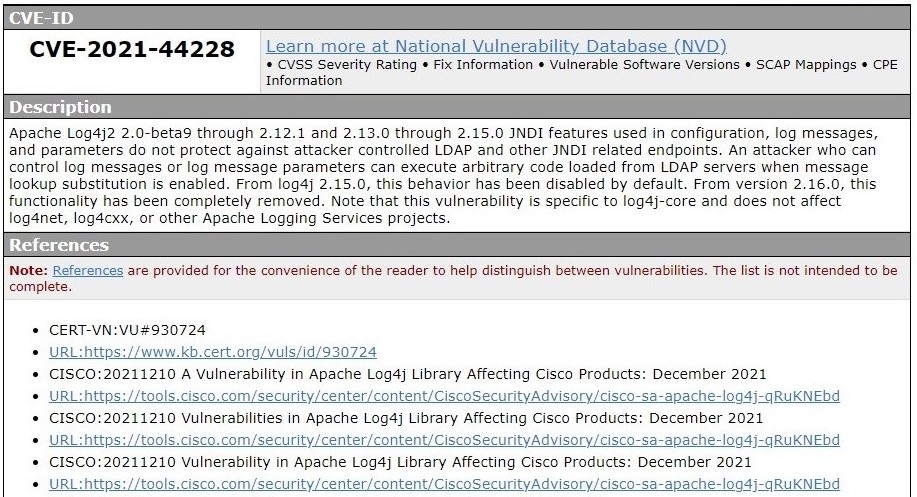
\includegraphics[width=0.98\textwidth]{fig/CVE-2021-44228-2}
    \caption{CVE平台中漏洞CVE-2021-44228}\label{fig:CVE-2021-44228}
\end{figure}

\begin{figure}[!t]
    \centering
    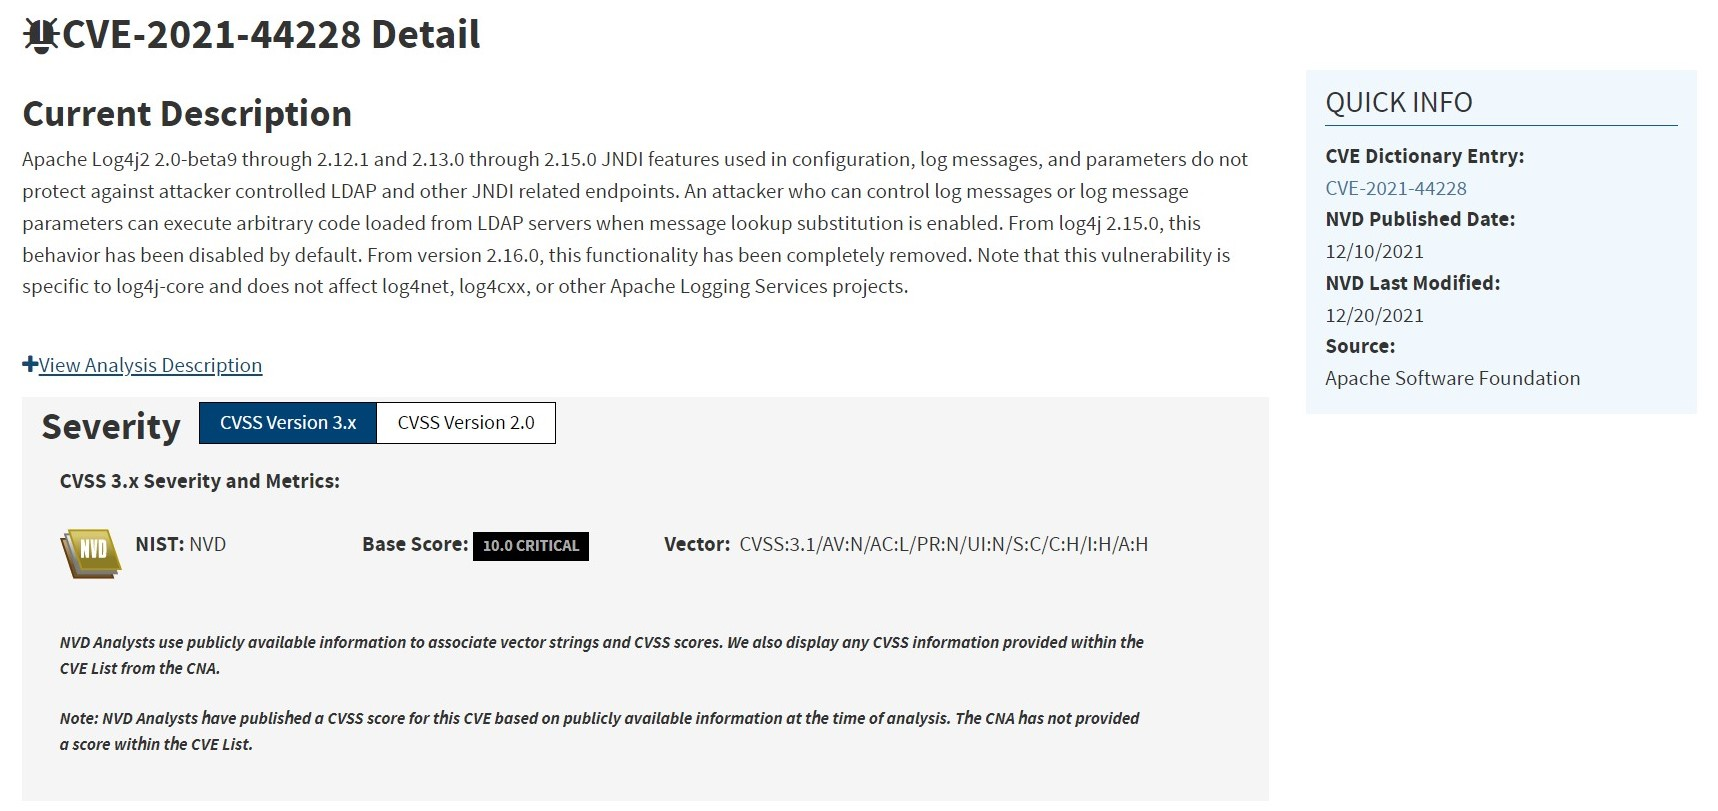
\includegraphics[width=1.0\textwidth]{fig/NVD-2021-44228}
    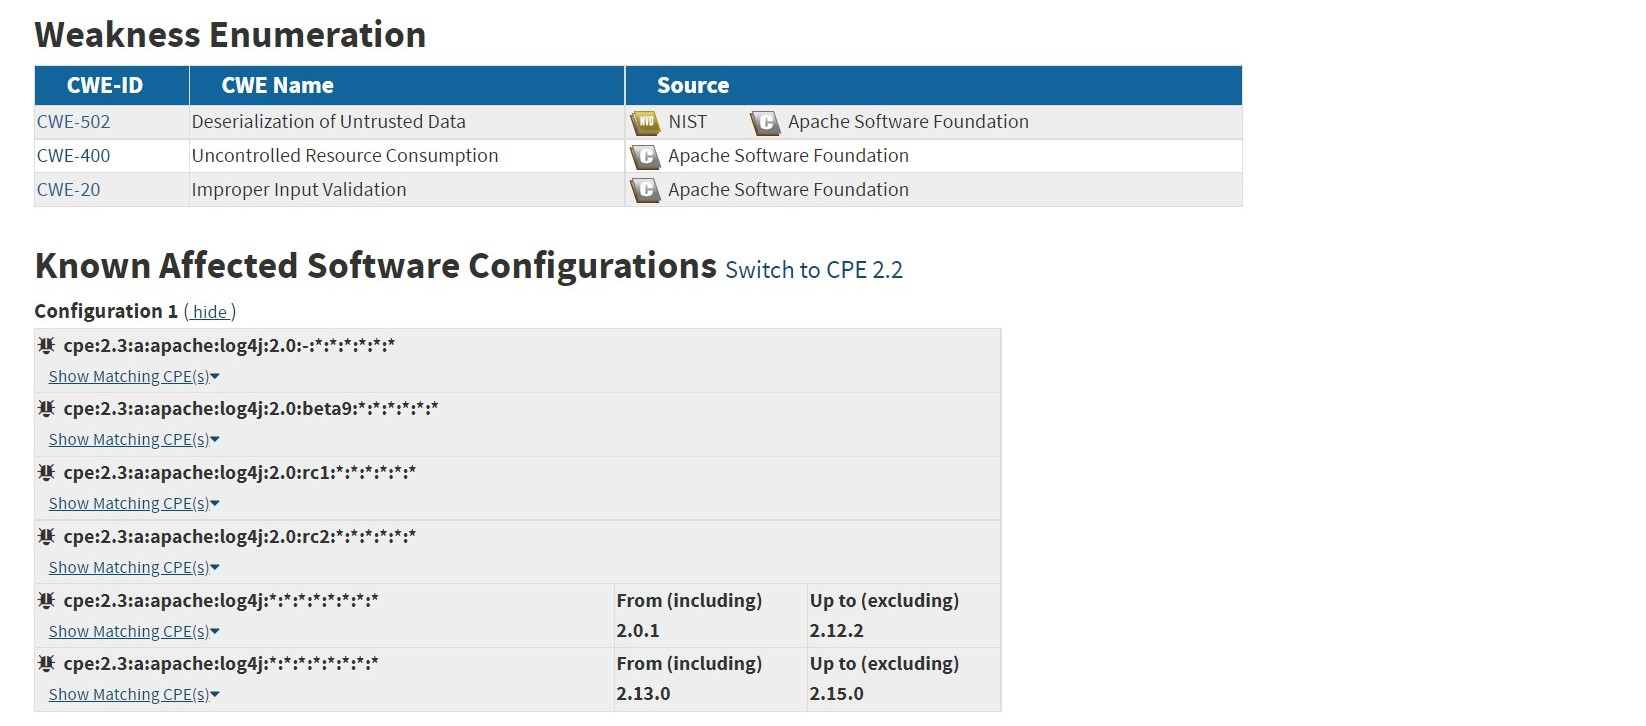
\includegraphics[width=1.0\textwidth]{fig/NVD-2021-44228-2}\caption{NVD平台中漏洞CVE-2021-44228}
    \label{fig:NVD-2021-44228}
\end{figure}

% \tocheck{可解释下CVE List,以及在NVD之后,描述下CVEdetails。}

CVE被设计作为漏洞字典用于收录并编号漏洞,这也导致CVE中漏洞信息过于精简,仅有一段漏洞描述和参考链接信息。基于CVE平台收录的漏洞条目信息,美国国家漏洞数据库(NVD)\footnote{https://nvd.nist.gov/}、中国国家信息安全漏洞库(CNNVD)\footnote{http://www.cnnvd.org.cn/}等漏洞数据库被构建。这些数据库与CVE平台数据完全同步,并为每个漏洞条目(CVE Entry)提供更丰富的信息,如:影响的软件名及版本、修复信息、严重性评分、影响评级等。图\ref{fig:NVD-2021-44228}所示为NVD平台中漏洞CVE-2021-44228\footnote{https://nvd.nist.gov/vuln/detail/CVE-2021-44228}。




\subsection{漏洞公告} 
% 是什么? 有哪些信息? 有哪些种(official、third-party)?举个例子?
漏洞公告(Advisory),也被称为漏洞通告,一般是由受漏洞影响的软件的厂商(Vendor)对外发布的安全漏洞警报,通常包含:漏洞触发描述、漏洞影响结果、漏洞软件名、软件版本等描述信息,有时也会包含漏洞发现者、漏洞问题报告(Issue Report)、漏洞补丁等知识。

\begin{figure}[!t]
    \centering
    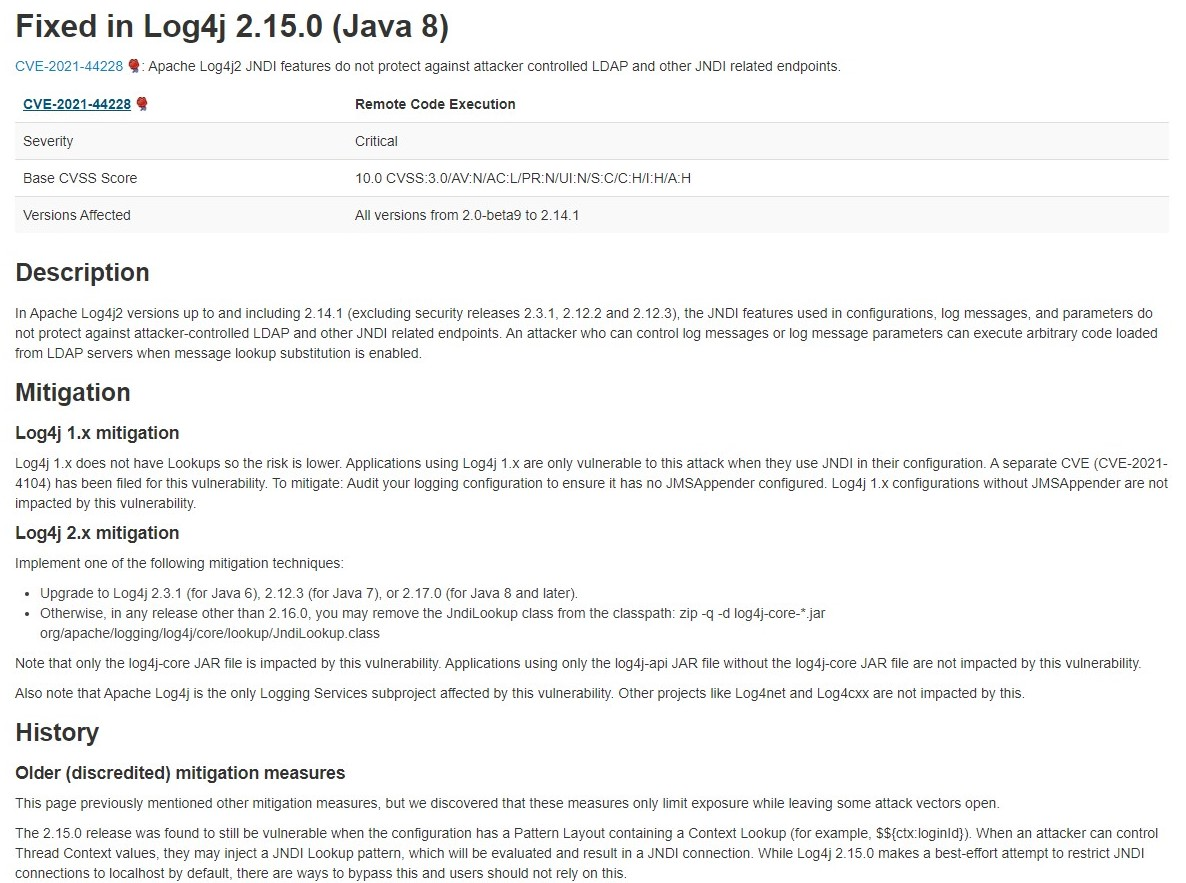
\includegraphics[width=1.0\textwidth]{fig/Vendor-2021-44228}
    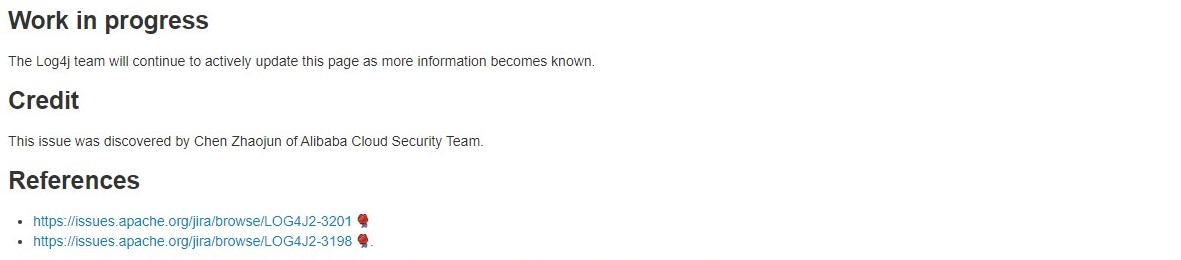
\includegraphics[width=1.0\textwidth]{fig/Vendor-2021-44228-2}
    \caption{Apache Log4j发布的漏洞CVE-2021-44228公告}
    \label{fig:Vendor-2021-44228}
\end{figure}

图\ref{fig:Vendor-2021-44228}为厂商Apache发布的关于安全漏洞CVE-2021-44228的公告\footnote{https://logging.apache.org/log4j/2.x/security.html},包含修复方式---“Log4j 2.x mitigation ...... Upgrade to Log4j 2.3.1 (for Java 6), 2.12.3 (for Java 7), or 2.17.0 (for Java 8 and later)”、漏洞发现者---“Credit:This issue was discovered by Chen Zhaojun of Alibaba Cloud Security Team.”、参考链接---“https://issues.apache.org/jira/browse/LOG4J2-3198”等信息。


以上介绍的由厂商发布的漏洞公告,也被称为:厂商公告(Vendor Advisory)。由于某一厂商只会发布、维护与该厂商相关的软件漏洞通告,而开源社区的开发人员难以一一关注所有厂商的公告信息,因此,出现了许多第三方平台致力于收集并维护所有漏洞公告信息。这些由第三方平台收集并维护的漏洞公告也被称为:第三方公告(Third-Party Advisory)。目前,认可度较高、影响力较大的第三方漏洞公告平台有Red Hat\footnote{https://access.redhat.com/errata/}、Debian\footnote{https://www.debian.org/security/}、Gentoo\footnote{https://security.gentoo.org/}等。

% 官方或第三方?再顺路引出相关的sources,作为例子。

% Vender advisory, official advisory:CVE NVD,third-party advisory:Redhat debian 啥啥
% 是什么? 有哪些信息? 有哪些种(official、third-party:权威或非权威啥啥啥。。。社区、工业啥啥、、、)?举个例子?

\begin{figure}[!t]
    \centering
    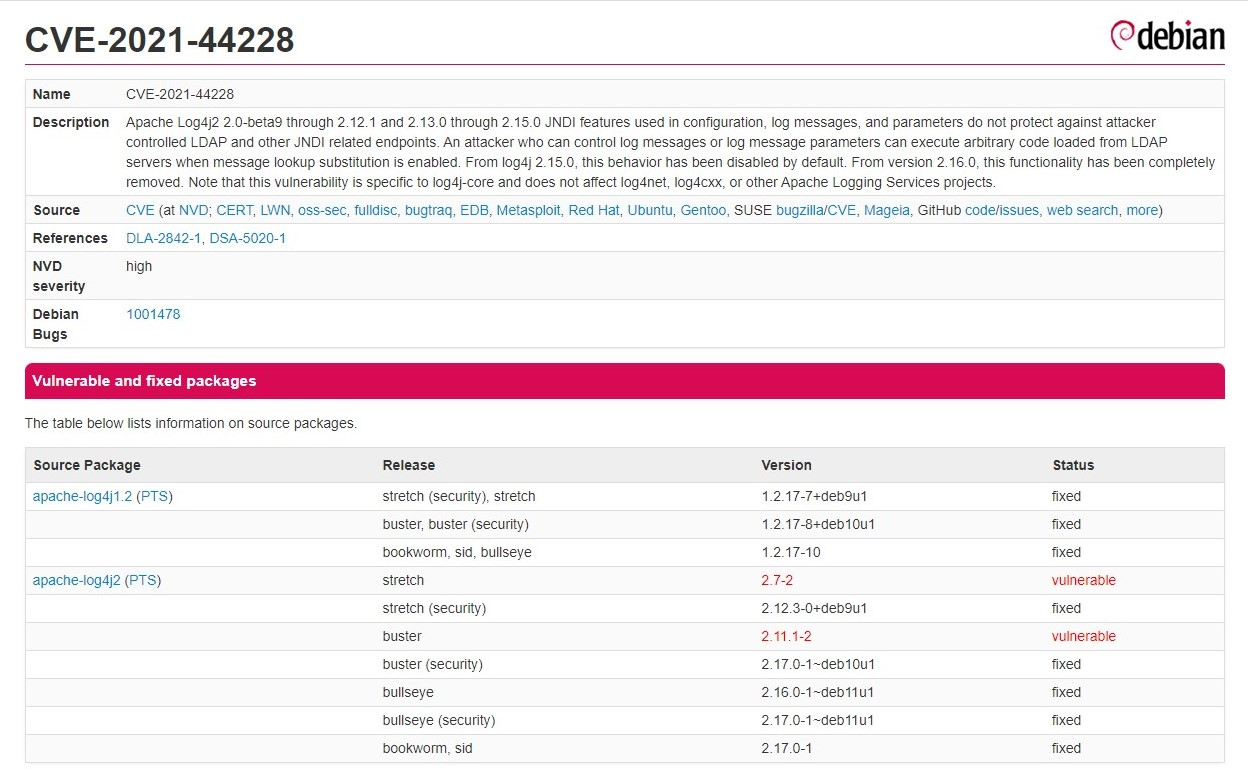
\includegraphics[width=1.0\textwidth]{fig/debian-2021-44228}
    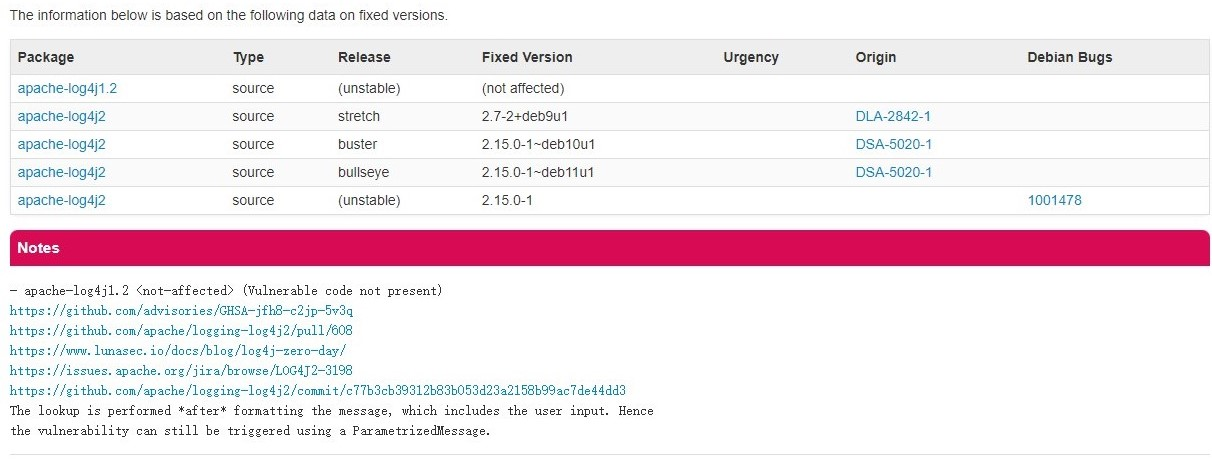
\includegraphics[width=1.0\textwidth]{fig/debian-2021-44228-2}
    \caption{Debian平台中漏洞CVE-2021-44228的公告}
    \label{fig:debian-2021-44228}
\end{figure}
图\ref{fig:debian-2021-44228}为Debian平台中漏洞CVE-2021-44228的公告\footnote{https://security-tracker.debian.org/tracker/CVE-2021-44228},其中还包括了该漏洞的补丁c77b3c@logging-log4j2\footnote{https://github.com/apache/logging-log4j2/commit/c77b3cb39312b83b053d23a2158b99ac7de44dd3}(即图中“Note”引用的参考链接),这在NVD和Vendor Advisory中都未出现。


\subsection{漏洞补丁}
补丁(Patch),也称:补丁程序,是指对计算机程序进行的一组更改,旨在更新其功能或修复其缺陷。漏洞补丁(Vulnerability Patch)则指为修复程序中的安全漏洞所开发的补丁,通常是Git和SVN中的代码提交(Commit),或是文本文件(.patch文件)形式。对于代码提交形式的补丁,后文中将简称为补丁提交。

\begin{figure}[!t]
    \centering
    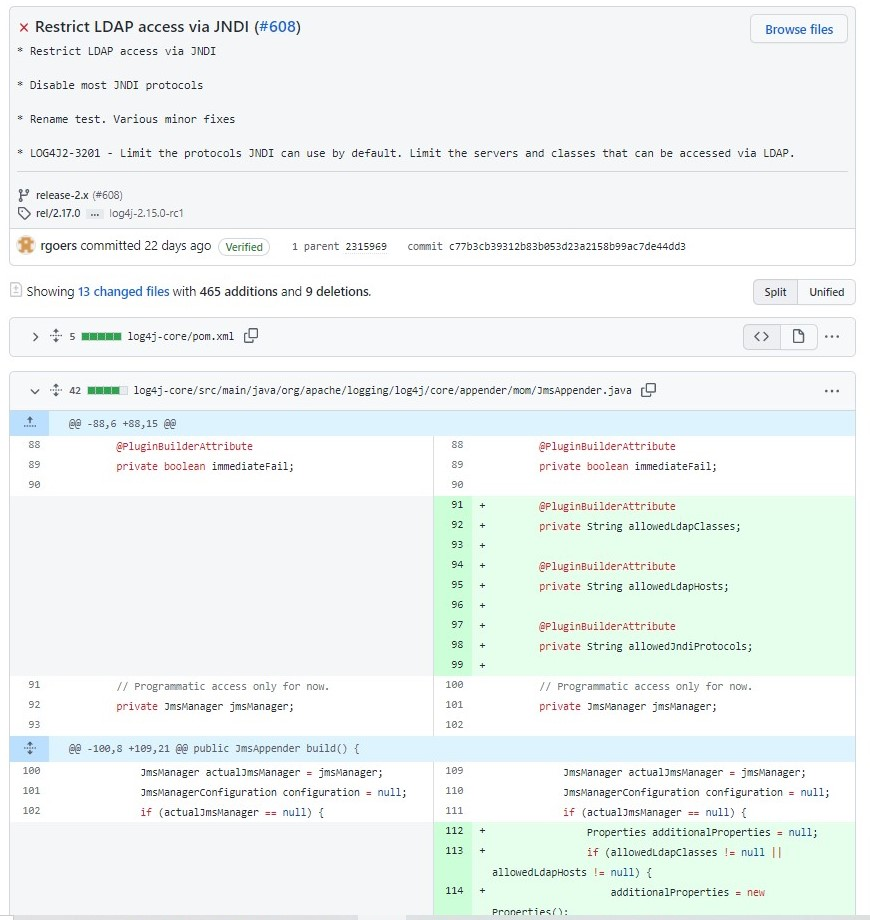
\includegraphics[width=0.95\textwidth]{fig/commit-2021-44228}
    \caption{漏洞CVE-2021-44228的Github Commit补丁}
    \label{fig:commit-2021-44228}
\end{figure}

例如,上图\ref{fig:debian-2021-44228}中的参考链接“https://github.com/apache/logging-log4j2/commit/\\c77b3cb39312b83b053d23a2158b99ac7de44dd3”,即为漏洞CVE-2021-44228的补丁提交,该提交的内容见图\ref{fig:commit-2021-44228}。


\section{相关工作}
\subsection{漏洞信息质量}
随着社区、工业界及学术界构建的漏洞数据库越来越多,数据库中积累的漏洞数据也越来越多,研究人员开始关注数据库中漏洞信息的质量。

Nguyen和Massacci\cite{nguyen2013reliability}最早揭示了NVD数据库中软件版本信息的不准确情况。为了提高这项信息的可靠性,Nguyen\cite{nguyen2016automatic}和Dashevskyi等人\cite{dashevskyi2018screening}提出方法,用以确定某一软件的旧版本是否会受到新披露漏洞的影响。他们认为:如果软件的旧版本包含修复漏洞所更改的代码行,则该版本被视为受新披露的漏洞影响。
不同于以上工作的方法,Dong等人\cite{dong2019towards}从漏洞的描述信息中识别受漏洞影响的软件名称和版本,并与漏洞报告所提供的软件名称和版本信息进行对比,以此发现不一致、不准确的软件版本信息。他们发现,NVD等多个漏洞数据库中会遗漏真正受漏洞影响的版本,也会错误地包含了不受漏洞影响的版本。

除了受漏洞影的软件版本信息,Mu等人\cite{mu2018understanding}揭示了漏洞报告中,普遍缺失用于重现漏洞的关键步骤。Chaparro等人\cite{chaparro2017detecting}提出方法用于检测漏洞描述中是否缺少用于重现漏洞的关键步骤及预期结果信息。以上工作主要侧重于漏洞的软件版本及漏洞重现的信息,而本文则重点关注漏洞数据库中的补丁知识,并尝试自动化地从多个知识源的漏洞公告信息中定位漏洞补丁。
% \tocheck{jo等人}\cite{jo2020gapfinder}识别网络安全领域内的语义不一致。
% \tocheck{这些工作侧重于漏洞信息的不同方面。按照这个方向,我们的工作重点是漏洞补丁,并尝试从漏洞报告的综合来源中识别漏洞补丁。}

Tan等人完成了一项与本文的研究问题较为相似的工作\cite{Tan2021locating}。他们使用深度学习排名算法对代码仓库中的代码提交进行排名,把排在首位的代码提交作为漏洞的补丁提交。他们的工作包含两个假设:(1)受漏洞影响的软件的代码仓库已知,(2)漏洞与其补丁提交在数量上是一对一的映射关系。然而,事实上,受漏洞影响的软件的代码仓库并不全部已知,而需人工识别。此外,漏洞与其补丁提交在数量上存在一对多的关系(见章节\ref{sec:cardinality})。所以,该方法对于开源软件漏洞不具有通用性。


% \subsection{漏洞补丁分析}
% 当前,有多中补丁分析相关的任务可用于提高软件安全性,如:补丁的生成和部署\cite{mulliner2013patchdroid,duan2019automating,xu2020automatic}、补丁的存在性测试\cite{zhang2018precise,jiang2020pdiff,dai2020bscout}以及秘密补丁识别\cite{xu2017spain,zhou2017automated,sabetta2018practical,chen2020machine}。

% 此外,研究人员也已为Java\cite{ponta2019manually}、C/C++\cite{fan2020ac}以及特定开源项目\cite{jimenez2018enabling}构建安全补丁数据集。基于这些数据集,研究人员已开展实证研究以表征漏洞及其补丁\cite{zaman2011security,li2017large,liu2020large,antal2020exploring}。在这些工作中,补丁多由人工识别\cite{xu2020automatic,jiang2020pdiff,dai2020bscout,xu2017spain,zhou2017automated,sabetta2018practical,chen2020machine,ponta2019manually,zaman2011security},或通过启发式规则识别,例如:在CVE的参考链接中查找补丁提交信息\cite{duan2019automating,fan2020ac,jimenez2018enabling,li2017large,liu2020large},以及在提交信息(Commit Message)中搜索CVE标识符\cite{fan2020ac, jimenez2018enabling, antal2020exploring}。这些工作存在的问题为:通过人工收集成本过高,且耗时较长;然而,启发式规则的方法又不足以找到或是找全补丁。

\subsection{漏洞补丁识别}
随着披露的开源软件漏洞越来越多、漏洞影响越来越大,为了能够及时获取补丁知识,许多自动化的补丁识别方法被提出。

周鹏等人\cite{9周鹏2022一种}提出了一种针对Linux内核的安全漏洞修复补丁自动识别方法,该方法通过持续收集并标注安全漏洞补丁数据,以及定义并抽取原始补丁文件的特征,来训练一个可识别安全漏洞修复补丁的分类器。邹雅毅等人\cite{7邹雅毅2016开源软件漏洞补丁的采集与整理}针对Linux内核、Ffmpeg、Wireshark三个项目设计了一种DIFF文件形式的补丁采集方法。该方法通过定义的DIFF特征来识别补丁链接,并基于与补丁链接出现在同一页面的CVE ID来完成漏洞及其修复补丁映射关系的确认。

李瑞科等人\cite{10李瑞科20191999}构建了一个包括近20年漏洞数据的安全漏洞数据集,通过程序自动化和人工采集结合的方法采集了多个国内外知名漏洞平台1999–2018年间的安全漏洞数据,并对采集的漏洞数据进行切片和格式化操作。Li和Vern\cite{li2017large}基于NVD平台的漏洞数据,通过收集带有Git代码提交链接的漏洞,实现漏洞补丁数据集的构建。同样,Liu等人\cite{liu2020large}也是基于CVE和NVD漏洞报告中参考链接的数据,解析并识别GitHub代码提交的链接作为漏洞补丁。Ponta等人\cite{ponta2019manually}通过人工手动收集的方式,构建一个针对Java语言,包含205个开源项目、624个漏洞、1282个补丁的数据集。

Fan等人\cite{fan2020ac}针对Google Chrome、 Linux和 Google Android项目构建了一个C及C++语言的漏洞数据集。通过分析CVE Details漏洞报告中带有Git仓库的参考链接,确定该漏洞所影响软件的仓库,并以CVE ID及Bug ID作为关键词在该仓库的代码提交历史中搜索修复该漏洞的补丁。类似地,Jimenez等人\cite{jimenez2018enabling}提出了一种自动补丁识别框架--VulData7,并构建了一个针对Linux Kernel、WireShark、OpenSSL和 SystemD四个项目的漏洞补丁数据集。该框架也是以CVE ID及Bug ID作为关键词在该仓库的代码提交历史中搜索修复该漏洞的补丁。

上述工作提出的补丁识别方法,多是通过基于启发式规则从漏洞公告的参考链接或项目的历史代码提交中识别补丁。这些方法多是针对特定的程序语言或项目而设计,较为局限,无法适用于所有安全漏洞。


\subsection{漏洞补丁应用}
漏洞补丁可被用于多种软件安全性任务。例如,补丁存在性检测\cite{8文琪2020}、基于漏洞补丁生成漏洞攻击程序\cite{brumley2008automatic,you2017semfuzz}、基于漏洞补丁进行漏洞影响分析\cite{4李舟军2015软件安全漏洞检测技术,5李韵2020基于机器学习的软件漏洞挖掘方法综述,pashchenko2018vulnerable,ponta2020detection,pashchenko2020vuln4real,Wang2020empirical} 以及基于漏洞补丁进行漏洞检测\cite{li2016vulpecker,li2018vuldeepecker,zhou2019devign,jimenez2019importance}。%、通过匹配漏洞签名\cite{jang2012redebug,kim2017vuddy}、通过匹配漏洞和补丁检测签名\cite{xu2020patch,xiao2020mvp,cui2020vuldetector}来检测程序中的漏洞。

文琪等人\cite{8文琪2020}提出一个名为PatchChecker的基于关键路径和语义的漏洞补丁存在性检测方法。该方法通过识别漏洞的修复路径及其程序修复前后的语义特征,生漏洞补丁的签名。基于补丁签名,在目标程序中识别对应路径并进行比较,以判断漏洞补丁是否被应用。%基于安全漏洞的补丁数据,Li等人\cite{[16]}提出了一种可扩展的漏洞检测方法,该方法使用一种可扩展的基于语法的方法来识别克隆的漏洞代码。
Li等人\cite{li2016vulpecker}提出了一种基于代码相似度分析的自动化漏洞检测方法。给定漏洞,该方法先抽取该漏洞补丁中的代码特征,再利用代码相似度算法检测项目中相似的代码,实现漏洞检测。之后,Li等人\cite{li2018vuldeepecker}又提出了一种基于深度学习系统的漏洞检测方法。Kim等人\cite{kim2017vuddy}提出了一种可扩展的克隆代码的安全漏洞检测方法。该方法利用函数级代码和基于长度过滤技术,能够高效准确地检测大型软件程序中的安全漏洞。

Xu等人\cite{xu2020patch}提出了一种名为BinXray基于补丁的漏洞匹配方法,以准确有效地识别程序中的“1-day”漏洞。该方法首先通过比较漏洞修复前后的程序,基于程序块轨迹来提取补丁的签名。检测时,基于补丁语义加快签名搜索,并通过计算程序轨迹的相似性识别目标程序是否已修补。Xiao等人\cite{xiao2020mvp}提出了一种检测重现漏洞(Recurring Vulnerability)的方法,MVP。 该方法基于使用程序切片从漏洞函数的句法及语义中提取漏洞和补丁签名;在检测阶段,如果目标函数与漏洞签名匹配成功,但与补丁签名匹配不成功,则被识别为潜在漏洞。李赞等人\cite{22李赞2018}提出了一种利用补丁来提高相似性检测准确性的漏洞发现方法。该方法基于漏洞补丁,通过程序切片技术去除漏洞函数中与漏洞无关的代码,并利用程序切片生成漏洞特征来检测漏洞。李元成等人\cite{23李元诚2020}提出一种基于深度聚类算法的软件源代码漏洞检测方法。该方法先通过构造软件代码属性图,遍历代码中API序列,并将其向量化;再以关键代码为中心进行聚类,根据聚类结果判断异常函数并匹配漏洞库,从而实现漏洞代码的检测。

本文提出的方法可以为以上补丁存在性检测、漏洞影响分析、漏洞挖掘等工作提供漏洞补丁知识。


%与上一小结的补丁分析工作类似,这些工作中的CVE补丁主要通过人工识别\cite{pashchenko2018vulnerable,ponta2020detection,pashchenko2020vuln4real,xiao2020mvp}、基于启发式规则的方法\cite{li2016vulpecker,li2018vuldeepecker,you2017semfuzz,Wang2020empirical,jimenez2019importance}或直接取自为特定项目建立CVE和补丁之间映射关系的安全公告\cite{jang2012redebug,kim2017vuddy,xu2020patch}。但是,人工识别的成本过高,而且基于启发式规则的方法找到或是找全补丁。